\chapter{Green Function Technique}
Now, we would solve the wave equations in equations~\eqref{eqn:vectorpotentialeqnwithlorentzguage} and~\eqref{eqn:scalarpotential} using a technique known as the \emph{Green Function Technique}\index{green function technique}. The Green function technique is applied in solving inhomogeneous ordinary differential equations which, in this case, is what we have. The Green function technique solves for the Green function, which is a scalar denoted by $G$ for the differential equations given. The Green function, $G$, is the impulse response of the differential equation. For the wave equation, the green function, $G$, is the spatial impulse response of the system which is described by the wave equations. When applying the Green function technique to the wave equations given, we are essentially solving for the spatial impulse response of the wave equations. The spatial impulse response of the wave equations is the solution to the wave equations. The solution to the wave equations is the fields $\vec{E}$ and $\vec{H}$. The wave equations from in equations~\eqref{eqn:vectorpotentialeqnwithlorentzguage} and~\eqref{eqn:scalarpotential} are given by:
\begin{align}
\nabla^{2}\bar{A}-\mu\bar{A} = -\mu\bar{J}
\label{eqn:vectorpotentialeqnwithlorentzguage_lec47}\\
\nabla^{2}V-\mu\epsilon\frac{\partial V}{\partial t} = -\frac{\rho}{\epsilon}
\label{eqn:scalarpotential_lec47}
\end{align}
Let us note that the Laplace operator is scalar (it operates on a scalar) which means it operates on each component of the $\bar{A}$ vector. So essentially replacing the vector $\bar{A}$ with a scalar is possible.
Points to note when using the technique:
\begin{enumerate}[(i)]
\item First, we replace in the differential equations~\eqref{eqn:vectorpotentialeqnwithlorentzguage_lec47} and~\eqref{eqn:scalarpotential_lec47}, the original function (in this case, $\bar{A}$ and $V$) with the Green function and replace the driving quantity (in this case $-\mu\bar{J}$ and $-\frac{\rho}{\epsilon}$) with the impulse function $\delta = f_{n}$(space).
\item Next, we convolve the solution of the Green function with the driving quantity to get the solution to the original function.
\end{enumerate}

\subsection{Green Function for the Vector Potential}
Before applying the Green function technique, we know that the fields $\vec{E}$ and $\vec{H}$ are time-varying fields and so, $\vec{A}$ is also a time-varying field and vary with respect to $e^{j\omega t}$, hence,
\begin{align*}
\partialderivative{}{t} \equiv j\omega\quad\text{and}\quad\partialderivative[2]{}{t} \equiv j\omega.j\omega = -\omega^{2}
\end{align*}
Therefore, factoring in the time quantity would give the following equation for the vector potential:
\begin{align}
\nabla^{2}\bar{A}-\omega^{2}\mu\bar{A} = -\mu\bar{J}
\label{eqn:vectorpotentialeqnwithlorentzguage_lec47_timevarying}
\end{align}
Recall from the wave equation, in an inbound medium,
\begin{align*}
\beta^{2} &= \omega^{2}\mu \varepsilon\\
\beta &= \omega\sqrt{\mu \varepsilon}\\
\beta &= \omega\sqrt{\mu_o \varepsilon_o}\quad\text{for free space}
\end{align*}
So, equation~\eqref{eqn:vectorpotentialeqnwithlorentzguage_lec47_timevarying} can be written as:
\begin{align*}
\nabla^{2}\bar{A}+\beta^{2}\bar{A} = -\mu\bar{J}
\end{align*}
Applying the Green function technique, then,
\begin{align*}
\nabla^{2}\bar{G}+\beta^{2}\bar{G} = \delta(\text{space})
\end{align*}
Solving the equation in the spherical coordinate system,
\begin{dmath*}
\partialderivative{}{r} \left(r^{2} \partialderivative{G}{r} \right) + \frac{1}{r^2 \sin \theta} \partialderivative{}{\theta}\left(\sin \theta \partialderivative{G}{\theta}\right) + \frac{1}{r^{2}\sin^{2}\theta} \partialderivative[2]{G}{\phi} + \beta^{2}G = \delta(r,\theta,\phi)
\end{dmath*}

Considering the source at the origin (impulse located at origin) simplifies the solution because at whatever direction in space, you see the same source which makes the solution for the equation spherically symmetric. Hence, $G$ is not a function of $\theta$ and $\phi$ and $\derivative{}{\theta} \equiv \derivative{}{\phi} = 0
$. Thus, the differential equation becomes:
\begin{equation}
\derivative{}{r}\left(r^{2}\derivative{G}{r}\right) +  \beta^{2}G = \delta(r)\footnotemark
\label{eqn:vectorpotentialeqnwithlorentzguage_lec47_sphericalcoordinates}
\end{equation}
\footnotetext{
Notice the partial derivatives are converted to full derivatives because $G = f_{n}(r)$ only.
}
Let's define a variable $\psi = rG$, such that,
\begin{align*}
&\derivative{\psi}{r} = r\derivative{G}{r} + G&\\
&\derivative{G}{r} = \frac{1}{r}{\derivative{\psi}{r} - G}&\\
&\text{and}&\\
&G = \frac{\psi}{r}&
\end{align*}
Substitute $G$ and $\derivative{G}{r}$ interms of $\psi$ in equation~\eqref{eqn:vectorpotentialeqnwithlorentzguage_lec47_sphericalcoordinates}:
\begin{align*}
\frac{1}{r^{2}}\derivative{}{r}\left(r^{2}
\left(\frac{1}{r}(\derivative{\psi}{r} - G) \right) \right) + \beta^{2}\frac{\psi}{r} &= \delta(r)\\
\frac{1}{r^{2}}\derivative{}{r}\left(r\derivative{\psi}{r} - rG \right) + \beta^{2}\frac{\psi}{r} &= \delta(r)\\
\frac{1}{r^{2}}\derivative{}{r}\left(r\derivative{\psi}{r} \right) - \frac{1}{r^{2}}\derivative{}{r}(rG) + \beta^{2}\frac{\psi}{r} &= \delta(r)\\
\frac{1}{r^{2}}\left(r\derivative[2]{\psi}{r} + \derivative{\psi}{r} \right) - \frac{1}{r^{2}}\derivative{\psi}{r} + \beta^{2}\frac{\psi}{r} &= \delta(r)\\
\frac{1}{r}\derivative[2]{\psi}{r} + \frac{1}{r^{2}}\derivative{\psi}{r} - \frac{1}{r^{2}}\derivative{\psi}{r} + \beta^{2}\frac{\psi}{r} &= \delta(r)\\
\frac{1}{r}\left(\derivative[2]{\psi}{r} + \beta^{2}\psi \right) = \delta(r)
\end{align*}
\begin{equation}
\derivative[2]{\psi}{r} + \beta^{2}\psi = \delta(r)\label{eqn:greenfunction}
\end{equation}
Equation~\eqref{eqn:greenfunction} has the solution $\psi = Ce^{-j\beta r} + De^{j\beta r}$. The two terms represent the travelling waves in the direction of $r$ and $r$ is always positive in the spherical coordinate system. The first term represents a wave which is travelling in all positive directions, i.e. away from the origin, while the second term represents a wave that is travelling in the negative $r$ direction but $r$ is always positive, so it represents a wave that is moving towards the origin. Since our source is at the origin and there is no energy source elsewhere in the medium, then this wave does not exist. The solution now reduces to:
\begin{align*}
\psi = Ce^{-j\beta r}
\end{align*}
But recall $G = \frac{\psi}{r}$, hence the solution for the Green function is:
\begin{align}
G = \frac{Ce^{-j\beta r}}{r}
\label{eqn:greenfunction_solution}
\end{align}
\begin{figure}[h]
\centering
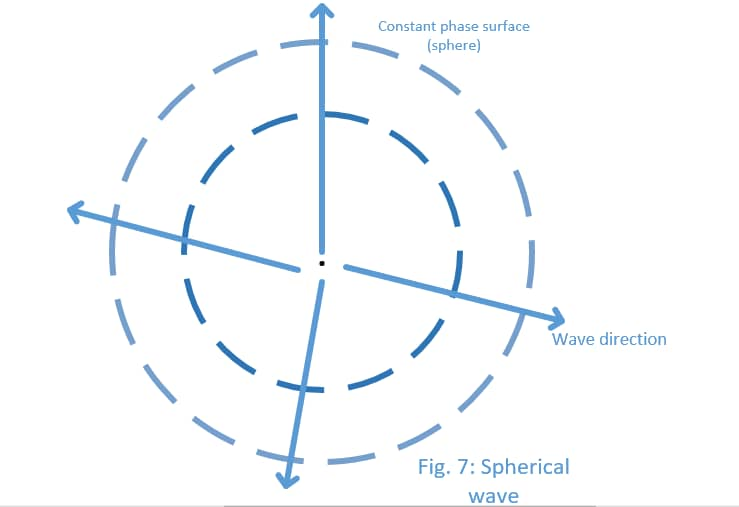
\includegraphics[width=\linewidth]{\pathtoparttwo/graphics/img_1}
\caption{Spherical wave}
\label{fig:sphericalwave}
\end{figure}

It should be noted that a constant $r$ represents the constant phase surface. In the spherical coordinate system when $r$ equals a constant, we know it represents a sphere so these constant phase surfaces are spheres and the wave propagating is called the \emph{spherical wave}\index{spherical wave}. Also, one other thing to be noted is that the amplitude of the spherical wave reduces by $\frac{1}{r}$ as opposed to the uniform plane wave in which the amplitude does not change as a function of space. In conclusion, the solution of the Green function, $G$, gives a spherical wave whose magnitude reduces by  $\frac{1}{r}$ and whose phase fronts are spheres.

\subsection{Solution of the Green function in the presence of a source}
The solution of the Green function in equation~\eqref{eqn:greenfunction_solution} is not complete as the solution is the impulse response which is the complementary solution of the differential equation, hence, let's compute $C$ by applying the appropriate boundary conditions.

To evaluate $C$, we substitute the general solution of $G = \frac{Ce^{-j\beta r}}{r}$ in the original differential equation in equation~\eqref{eqn:vectorpotentialeqnwithlorentzguage_lec47_sphericalcoordinates}, integrate the whole expression over the volume around the origin, and then take a limit when $r\rightarrow0$\footnote{
We take the limit when $r\rightarrow0$ because the source is at the origin. Also note that generally the limit is taken for an impulse response, but in this case, the source is at the origin, so the limit is taken when $r\rightarrow0$.
}
\begin{dmath*}
\lim\limits_{r\rightarrow0} \left\lbrace \int_{0}^{r} \int_{0}^{\pi}\int_{0}^{2\pi}\frac{1}{r^{2}}\derivative{}{r}\left[{r^{2}}\derivative{}{r}\left[\frac{Ce^{-j\beta r}}{r}\right]\right]r^{2}\sin\theta dr d\theta d\phi + \beta^{2} \int_{0}^{r} \int_{0}^{\pi}\int_{0}^{2\pi}\frac{Ce^{-j\beta r}}{r}r^{2}\sin\theta drd\theta d\phi\right\rbrace
= \lim\limits_{r\rightarrow0}\int_{v}\delta(r)dr
\end{dmath*}
% \begin{dmath*}
% \lim\limits_{r\rightarrow0} \int_{0}^{r} \int_{0}^{\pi}(2\pi)\derivative{}{r}\left[{r^{2}}\derivative{}{r}\left[\frac{Ce^{-j\beta r}}{r}\right]\right]\sin\theta d\theta dr + \beta^{2} \int_{0}^{r} \int_{0}^{\pi}(2\pi)\sin\theta d\theta[rCe^{-j\beta r}]dr = 1
% \end{dmath*}
% \begin{dmath*}
% \lim\limits_{r\rightarrow0} \left[4\pi\int_{0}^{r}\derivative{}{r}\left[{r^{2}}\derivative{}{r}\left[\frac{Ce^{-j\beta r}}{r}\right]\right]dr + C\beta^{2}4\pi\int_{0}^{r}re^{-j\beta r}dr\right] = 1
% \end{dmath*}
\begin{dmath*}
\lim\limits_{r\rightarrow0}\left\lbrace 4\pi\footnotemark C\int_{0}^{r}\derivative{}{r}\left[{r^{2}}\derivative{}{r}\left[\frac{e^{-j\beta r}}{r}\right]\right]dr + 4\pi C\beta^{2}\int_{0}^{r}re^{-j\beta r}dr \right\rbrace = 1\footnotemark
\end{dmath*}
\footnotetext{
The integration of the terms of the differential equation has been done in the $\theta$ and $\phi$ directions and the result is $4\pi$.
}
\footnotetext{
The limit of the volume integral of the delta function is $1$ because the volume integral of the delta function is the charge density, $\rho$, and the charge density is $1$ at the origin.
}
\begin{dmath*}
\lim\limits_{r\rightarrow0}\left\lbrace4\pi C\int_{0}^{r}\derivative{}{r}\left[{r^{2}}\left[\frac{r(-j\beta e^{-j\beta r}) - e^{-j\beta r}}{r^{2}}\right]\right]dr + 4\pi C\beta^{2}\int_{0}^{r}re^{-j\beta r}dr \right\rbrace = 1
\end{dmath*}
\begin{dmath*}
\lim\limits_{r\rightarrow0} \left\lbrace4\pi C\int_{0}^{r}\derivative{}{r}\left(-jr\beta e^{-j\beta r} - e^{-j\beta r}\right)dr + 4\pi C\beta^{2}\int_{0}^{r}re^{-j\beta r}dr\right\rbrace = 1
\end{dmath*}
\begin{dmath*}
\lim\limits_{r\rightarrow0} \left\lbrace4\pi C\int_{0}^{r}-\derivative{}{r}\left( e^{-j\beta r} (j\beta r + 1)\right)dr + 4\pi C\beta^{2}\int_{0}^{r}re^{-j\beta r}dr\right\rbrace = 1
\end{dmath*}
\begin{dmath*}
\lim\limits_{r\rightarrow0} \left\lbrace4\pi C\int_{0}^{r}-(e^{-j\beta r}\times j\beta + (j\beta r + 1)\times -j\beta e^{-j\beta r})dr + 4\pi C\beta^{2}\int_{0}^{r}re^{-j\beta r}dr\right\rbrace = 1
\end{dmath*}
\begin{dmath*}
\lim\limits_{r\rightarrow0} \left\lbrace4\pi C\int_{0}^{r}-(e^{-j\beta r} (j\beta + \beta^2r - j\beta))dr + 4\pi C\beta^{2}\int_{0}^{r}re^{-j\beta r}dr\right\rbrace = 1
\end{dmath*}
\begin{dmath*}
\lim\limits_{r\rightarrow0} \left\lbrace4\pi C\int_{0}^{r}-(\beta^2r e^{-j\beta r})dr + 4\pi C\beta^{2}\int_{0}^{r}re^{-j\beta r}dr\right\rbrace = 1
\end{dmath*}
\begin{align*}
\text{Let, }u = r\quad dv=e^{-j\beta r}dr\\
\text{then, }du=dr\quad v=j\frac{e^{-j\beta r}}{\beta}
\end{align*}
\begin{dmath*}
\lim\limits_{r\rightarrow0} \left\lbrace-4\pi C\beta^{2}\left[j\frac{re^{-j\beta r}}{\beta}\bigg\vert_{0}^{r}\frac{-j}{\beta}\int_{0}^{r}e^{-j\beta r}dr\right] + 4\pi C\beta^{2}\int_{0}^{r}re^{-j\beta r}dr\right\rbrace = 1
\end{dmath*}
% \begin{dmath*}
% \lim\limits_{r\rightarrow0} \left\lbrace-4\pi C\beta^{2}\left[j\frac{re^{-j\beta r}}{\beta}  \frac{-j}{\beta}\left(j\frac{e^{-j\beta r}}{\beta}\right)\right] + 4\pi C\beta^{2}\int_{0}^{r}re^{-j\beta r}dr\right\rbrace = 1
% \end{dmath*}
% \begin{dmath*}
% \lim\limits_{r\rightarrow0} \left\lbrace-4\pi C\beta^{2}\left[j\frac{re^{-j\beta r}}{\beta}  +\frac{e^{-j\beta r}}{\beta^{2}}\right] + 4\pi C\beta^{2}\int_{0}^{r}re^{-j\beta r}dr\right\rbrace = 1
% \end{dmath*}
\begin{dmath*}
\lim\limits_{r\rightarrow0} \left\lbrace-4\pi C e^{-j\beta r}\left[j\frac{r\beta^{2}}{\beta} +\frac{\beta^{2}}{\beta^{2}}\right] + 4\pi C\beta^{2}\int_{0}^{r}re^{-j\beta r}dr\right\rbrace = 1
\end{dmath*}
\begin{dmath*}
\lim\limits_{r\rightarrow0} \left\lbrace-4\pi C e^{-j\beta r}(j\beta r+1) + 4\pi C\beta^{2}\int_{0}^{r}re^{-j\beta r}dr\right\rbrace = 1
\end{dmath*}
Taking limit $r\rightarrow0$ gives
$$-4\pi C= 1$$
$$C = \frac{-1}{4\pi}$$
Hence, the complementary solution of the Green function is given as $ G= -\frac{e^{-j\beta r}}{4\pi r}$
With the impulse response, G we can find the solution to $\vec{A}$ which is the convolution of the impulse response with the driving function.

Hence, 
\begin{equation}
\vec{A}=\int_{v}\mu\vec{J}(r^{'}) \frac{e^{-j\beta\vert\vec{r}-\vec{r^{'}}\vert}}{4\pi|\vec{r}-\vec{r^{'}}|}dV'
\label{eqn:vector_potential_complete}
\end{equation}
which is the convolution integral. $\vec{r^{'}}$ denotes the position vector of the location of the current, while r is the position vector of the location where we are computing the vector potential. The expression can be best understood by considering figure~\ref{fig:img_2}, where there is a region where the source is located, denoted by $\vec{J}(r')$, for an infinitesimal volume, $dV^{'}$, the current is given by $\vec{J}(r')dV$.
\begin{figure}[h]
\centering
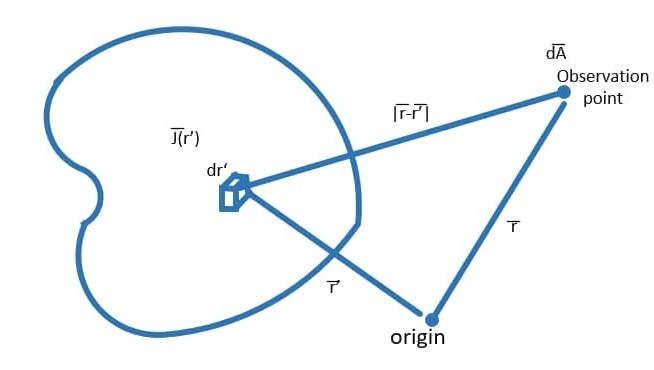
\includegraphics[width=0.8\linewidth]{\pathtoparttwo/graphics/img_2}
\caption{Illustration of the vector potential}
\label{fig:img_2}
\end{figure}

Also, there is one observation point where the vector potential is to be determined. The contribution of the vector potential, dA from the infinitesimal volume is given by: 
\begin{equation}
\mu\vec{J}(r^{'}) \frac{e^{-j\beta|\vec{r}-\vec{r^{'}}|}}{4\pi|\vec{r}-\vec{r^{'}}|}dV',
\end{equation}
So integrating it over the region of the space where the source is, gives the total vector potential given by equation~\eqref{eqn:vector_potential_complete}. The reason for the mod sign in equation~\eqref{eqn:vector_potential_complete} is to always have a positive value of r. So with the current distribution at the location $\vec{r^{'}}$, the magnetic vector potential at any point $\vec{r}$ can be calculated.

In this course, when modelling antennas, we assume the current distribution is given before the problem and our solution is simplified to just solving for the fields. However, if the current distribution were not given, then with some excitation point on the structure, the solution to the problem can be gotten from Maxwell's equation. But like it was said earlier, the current distribution is assumed to be given.
